\section{Large scale adaptive binding free energy calculations}

To enable the running of large amounts of simulations on supercomputers we developed the high throughput binding affinity calculator (HTBAC). The architecture of HTBAC and its uses is described here, and published in more detail in the proceedings of the 2018 eScience IEEE conference.
 
HTBAC is a software system for running ensemble-based free energy protocols
adaptively and at scale on HPC resources. Currently, HTBAC supports protocols
composed of an arbitrary number of analysis and simulation steps, and relies
on the ensemble management system and runtime system provided by the
RADICAL-Cybertools (RCT). HTBAC is designed to be extended to support more
types of protocols and alternative runtime middleware.

\subsection{Design and implementation}

HTBAC exposes four constructs to specify free energy protocols: Protocol,
Simulation, Analysis, and Resource. \textbf{Protocol} enables multiple
descriptions of protocol types, while \textbf{Simulation} and
\textbf{Analysis} specify simulation and analysis parameters for each
protocol. \textbf{Resource} allows to specify the amount of resources needed
to execute the given protocols.

In HTBAC, each protocol models a unique protein ligand physical system. Each
protocol follows a sequence of simulation and analysis steps, assigning
ensemble members to execute independent simulations or analysis. An ensemble
member that executes an independent simulation within a simulation step is
referred to as a replica. Each simulation is assigned a different initial
velocity, which enables simulations to begin in different parts of the
ligand's phase space.

Individual simulations or analyses with input, output, termination criteria
and dedicated resources are designed as a computational
\textbf{task}~\cite{power-of-many17}. Aggregates of tasks with dependencies
that determine the order of their execution constitute a \textbf{workflow}.
In this way, HTBAC encodes $N_P$ instances of the P$^{th}$ protocol as a
workflow of computational tasks.

Figure~\ref{fig:htbac} shows the components and subcomponents of HTBAC.
HTBAC API enables users to codify protocol descriptions in terms of protocol
type, simulation and analysis steps, and computer infrastructure
requirements. Descriptor uses two subcomponents to aggregate protocol
descriptions into a single application and resource description. Note that
Descriptor can aggregate different types of protocols, with different
computing and resource requirements.

Runner has three subcomponents: Execution Manager, Middleware Connector and
Runtime Adaptive Evaluator. Execution Manager communicates with the
execution layer via a connector to coordinate the execution of the
application. In principle, HTBAC can use multiple connectors for diverse
middleware to access different computing infrastructures.

Middleware Connector converts the application description of HTBAC into a
middleware-specific format. Execution Manager can pass the given application
to the connector in full or only in parts. This enables to start the
execution of an application before its full description is available or to
change those parts of the application that still have to be executed. This
will enable future capabilities like, for example, to concurrently execute
the application on diverse middleware.

Runtime Adaptive Evaluator enables the execution of adaptive applications.
This subcomponent can evaluate partial results of an application execution
via tailored algorithms. On the base of this evaluation, Runtime Adaptive
Evaluator can decide to return the control to Execution Manager or to modify
the description of the application that is being executed. In this way, HTBAC
implements adaptivity for diverse protocols, allowing users to define
arbitrary conditions and algorithms.

HTBAC is implemented in Python as a domain-specific library. All components
of HTBAC are implemented as objects that communicate via method calls. HTBAC
uses two RCT as building blocks~\cite{review_bb_2016}: Ensemble Toolkit
(EnTK) and RADICAL-Pilot (RP).

EnTK provides HTBAC capabilities to execute ensemble-based
applications~\cite{power-of-many17}. EnTK exposes three constructs:
\textbf{Task}, \textbf{Stage} and \textbf{Pipeline}. Tasks contain
information regarding an executable, its software environment and its data
dependencies. Stages are sets of tasks without mutual dependencies that can
execute concurrently. Pipeline are lists of stages, where stages can execute
only sequentially and each pipeline can execute independently. HTBAC uses a
Middleware Connector for EnTK to encode a protocol instance as a single
pipeline that contains stages of individual simulations and analyses tasks.

EnTK uses RP to execute tasks via pilots. RP supports task-level parallelism
and high-throughput by acquiring resources from a computing infrastructure
and scheduling tasks on those resources for execution. Pilot systems execute
tasks directly on the resources, without queuing them on the infrastructure's
scheduler.

\subsection{Adaptivity}

The design of HTBAC permits enhancing protocols while continuing to use
``static'' simulation engines. To this end, we implemented two adaptive
methods using HTBAC: adaptive quadrature and adaptive termination. Both of
these methods use the features of adaptivity offered in HTBAC to scale to
large number of concurrent simulations and to increase convergence rate and
obtain more accurate scientific results.

The aim of introducing adaptive quadrature for alchemical free energy
calculation protocols (e.g., TIES) is to reduce time to completion while
maintaining (or increasing) the accuracy of the results. Time to completion
is measured by the number of core hours consumed by the simulations. Accuracy
is defined as the error with respect to a reference value, calculated via a
dense $\lambda$ window spacing (65 windows). This reference value is used to
establish the accuracy of the non-adaptive protocol (which has 13 $\lambda$
windows) and the adaptive protocol (which has a variable number of $\lambda$
windows, determined at run time).

One of the input parameters of the adaptive quadrature algorithm is the
desired acceptable error threshold of the estimated integral. We set this
threshold to the error of the non-adaptive algorithm calculated via the
reference value. The algorithm then tries to minimise the number of $\lambda$
windows constrained by the accuracy requirement.

\begin{figure}
  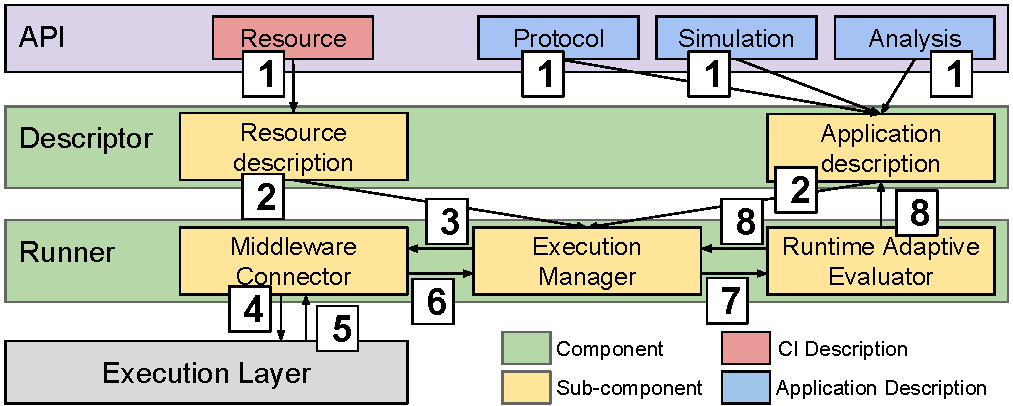
\includegraphics[width=\columnwidth]{HTBAC_architecture_model}
  \caption{HTBAC architecture. Users specify protocol(s) with multiple simulation and analysis steps. Descriptor derives a single application that Runner executes on an external execution layer. Runtime Adaptive Evaluator enables the execution of adaptive protocols.}
  \label{fig:htbac}
\end{figure}